\documentclass[runningheads]{llncs}
\usepackage[T1]{fontenc}
\usepackage{graphicx}
\usepackage{booktabs}

\begin{document}

\title{Improving Neural Collaborative Filtering through Ablation Studies on Model Architectures and Negative Sampling Strategies}

\titlerunning{Improving Neural Collaborative Filtering}

\author{Benard Adala Wanyande\orcidID{s4581733} \and Ataklti Haileslase\orcidID{s4590821}}

\authorrunning{B. A. Wanyande and A. Haileslase}

\institute{Leiden Institute of Advanced Computer Science, Leiden University, Leiden, Netherlands}

\maketitle

\begin{abstract}
This study aims to investigate the performance of Neural Collaborative Filtering (NCF) by exploring various model architectures and negative sampling strategies. Initial tests were conducted by varying the neural network configurations. Although these tests yielded minor improvements, further enhancements were pursued. Finally, an ablation study was performed to evaluate the effects of different negative sampling ratios on NCF performance, based on the following metrics: Hit Rate@10, NDCG@10, and Recall@10.
\end{abstract}

\section{Introduction}
Neural Collaborative Filtering (NCF) is a recommendation model that leverages deep learning by replacing traditional inner product operations with neural networks~\cite{he2017neural}. In particular, it integrates Generalized Matrix Factorization (GMF)\cite{he2017neural} and Multi-Layer Perceptrons (MLPs)\cite{he2017neural} to learn intricate, higher-dimensional user-item relationships. This allows for richer and more expressive latent representations compared to traditional linear collaborative filtering methods~\cite{koren2009matrix}.

\section{Research Methodology}
Initially, we implemented and evaluated a baseline NCF model (embedding dimension of 32, MLP layers [64, 32, 16, 8]), using a negative sampling ratio of 1:4. We hypothesized that varying the model's embedding dimensions (24, 32, 64, and 128) would yield significant performance improvements; however, these architectural adjustments provided incremental insights but did not notably enhance Recall@10. Given the limited gains from altering embedding sizes, we turned our focus to data-level adjustments, specifically negative sampling strategies. Inspired by Rendle et al.~\cite{rendle2012bpr}, we recognized that increasing the negative sampling ratio could improve the model's discrimination capabilities between positive and negative interactions. Thus, we performed an ablation study exploring multiple negative sampling ratios: 1:4 (baseline), 1:8, 1:10, 1:15, 1:50, and 1:100.

\section{Experimental Setup}

\subsection{Dataset and Initial Preprocessing}
For this study, we used the MovieLens dataset~\cite{harper2015movielens}. The initial preprocessing involved loading the dataset, which contained explicit ratings ranging from 0 to 5. We converted these explicit ratings into implicit feedback by mapping ratings greater than 4 to positive feedback ("1") and treating unrated movies as negative feedback ("0"). To generate negative feedback, we identified movies that users had not rated. For our baseline configurations, prior to the ablation tests, we sampled negative instances at a ratio of 1:4 (positive to negative).

\subsection{Model Implementation}
All models were implemented using PyTorch and trained using binary cross-entropy (BCE) loss, optimized with Adam, and employed early stopping to prevent overfitting.

\subsection{Evaluation Metrics}
We used the following standard metrics for evaluation~\cite{he2020lightgcn}:

\begin{itemize}
    \item \textbf{Hit Rate@10}
    \item \textbf{NDCG@10}
    \item \textbf{Recall@10}
\end{itemize}

\section{Results and Analysis}

\subsection{Impact of Embedding Dimensions on NCF Performance}

We initially explored the effects of varying embedding dimensions on the performance of Neural Collaborative Filtering (NCF) models. 

\begin{table}[h!]
\centering
\caption{Comparison of NCF Model Architectures with Varying Embedding Dimensions. Metrics include Hit Rate@10, NDCG@10, and Recall@10.}
\label{tab:results}
\begin{tabular}{lccc}
\toprule
\textbf{Embedding Dim.} & \textbf{Hit Rate@10} & \textbf{NDCG@10} & \textbf{Recall@10} \\
\midrule
32 (Baseline) & 0.9504 & 0.4882 & 0.4429 \\
64 & 0.9495 & 0.4908 & 0.4414 \\
128 & 0.9507 & 0.4933 & 0.4373 \\
24 & 0.9478 & 0.4806 & 0.4381 \\
\bottomrule
\end{tabular}
\end{table}

The embedding dimension of \underline{128} achieved the highest NDCG@10 (\underline{0.4933}), while the baseline \underline{32} yielded the best Recall@10 (\underline{0.4429}). These marginal differences suggest that increasing embedding size offers limited benefit, highlighting the need to explore data-level strategies like negative sampling.

\subsection{Negative Sampling Ablation Study}

We conducted an ablation study to investigate the impact of negative sampling ratios on the performance of Neural Collaborative Filtering (NCF) models. Adjusting negative sampling ratios is an essential data-level strategy for improving the model's ability to differentiate between positive and negative user-item interactions. Table~\ref{tab:negative_sampling_results} summarizes our findings from varying negative sampling ratios.

\begin{table}[h!]
\centering
\caption{Performance Comparison of NCF Models with Various Negative Sampling Ratios. Metrics evaluated are Hit Rate@10, NDCG@10, and Recall@10.}
\label{tab:negative_sampling_results}
\begin{tabular}{lccc}
\toprule
\textbf{Negative Ratio} & \textbf{Hit Rate@10} & \textbf{NDCG@10} & \textbf{Recall@10} \\
\midrule
1:4 (Baseline) & 0.9824 & 0.5112 & 0.5785 \\
1:8 & \underline{0.9872} & \underline{0.5178} & \underline{0.5916} \\
1:10 & 0.9802 & 0.5176 & 0.5775 \\
1:15 & 0.9787 & 0.5107 & 0.5695 \\
1:50 & 0.9724 & 0.4985 & 0.5531 \\
1:100 & 0.9653 & 0.4872 & 0.5418 \\
\bottomrule
\end{tabular}
\end{table}

The negative sampling ratio of \underline{1:8} yielded the best performance across all metrics—Hit Rate@10 (\underline{0.9872}), NDCG@10 (\underline{0.5178}), and Recall@10 (\underline{0.5916}). Beyond this point, performance declined with higher ratios (e.g., 1:50, 1:100), suggesting that too many negative samples may introduce noise. Thus, a moderate ratio like 1:8 offers an effective balance between discrimination and accuracy.

\section{Discussion}
Adjusting model complexity alone provided limited improvement, indicating diminishing returns from increased embedding dimensionality~\cite{he2017neural}. However, increasing the negative sampling ratio notably improved performance metrics, particularly Recall@10. The embedding dimension results suggest that beyond a certain complexity (32 in this study), further increases yield marginal gains, highlighting the importance of selecting appropriate model complexity. Conversely, the negative sampling ratio ablation emphasizes that a moderate ratio, such as 1:8, achieves optimal discrimination between positive and negative user-item interactions. Excessively high negative ratios introduce noise, reducing predictive accuracy, thereby underscoring the value of balanced negative sampling strategies in collaborative filtering tasks.

\section{Conclusion}
Our findings highlight the effectiveness of negative sampling adjustments in enhancing recommendation metrics, particularly recall. Future research should investigate advanced techniques such as regularization and hard negative mining to further improve recommendation systems~\cite{rendle2012bpr}.


\bibliographystyle{splncs04}
\bibliography{mybibliography}
\appendix

\section*{Appendix}

\begin{figure}[h!]
    \centering
    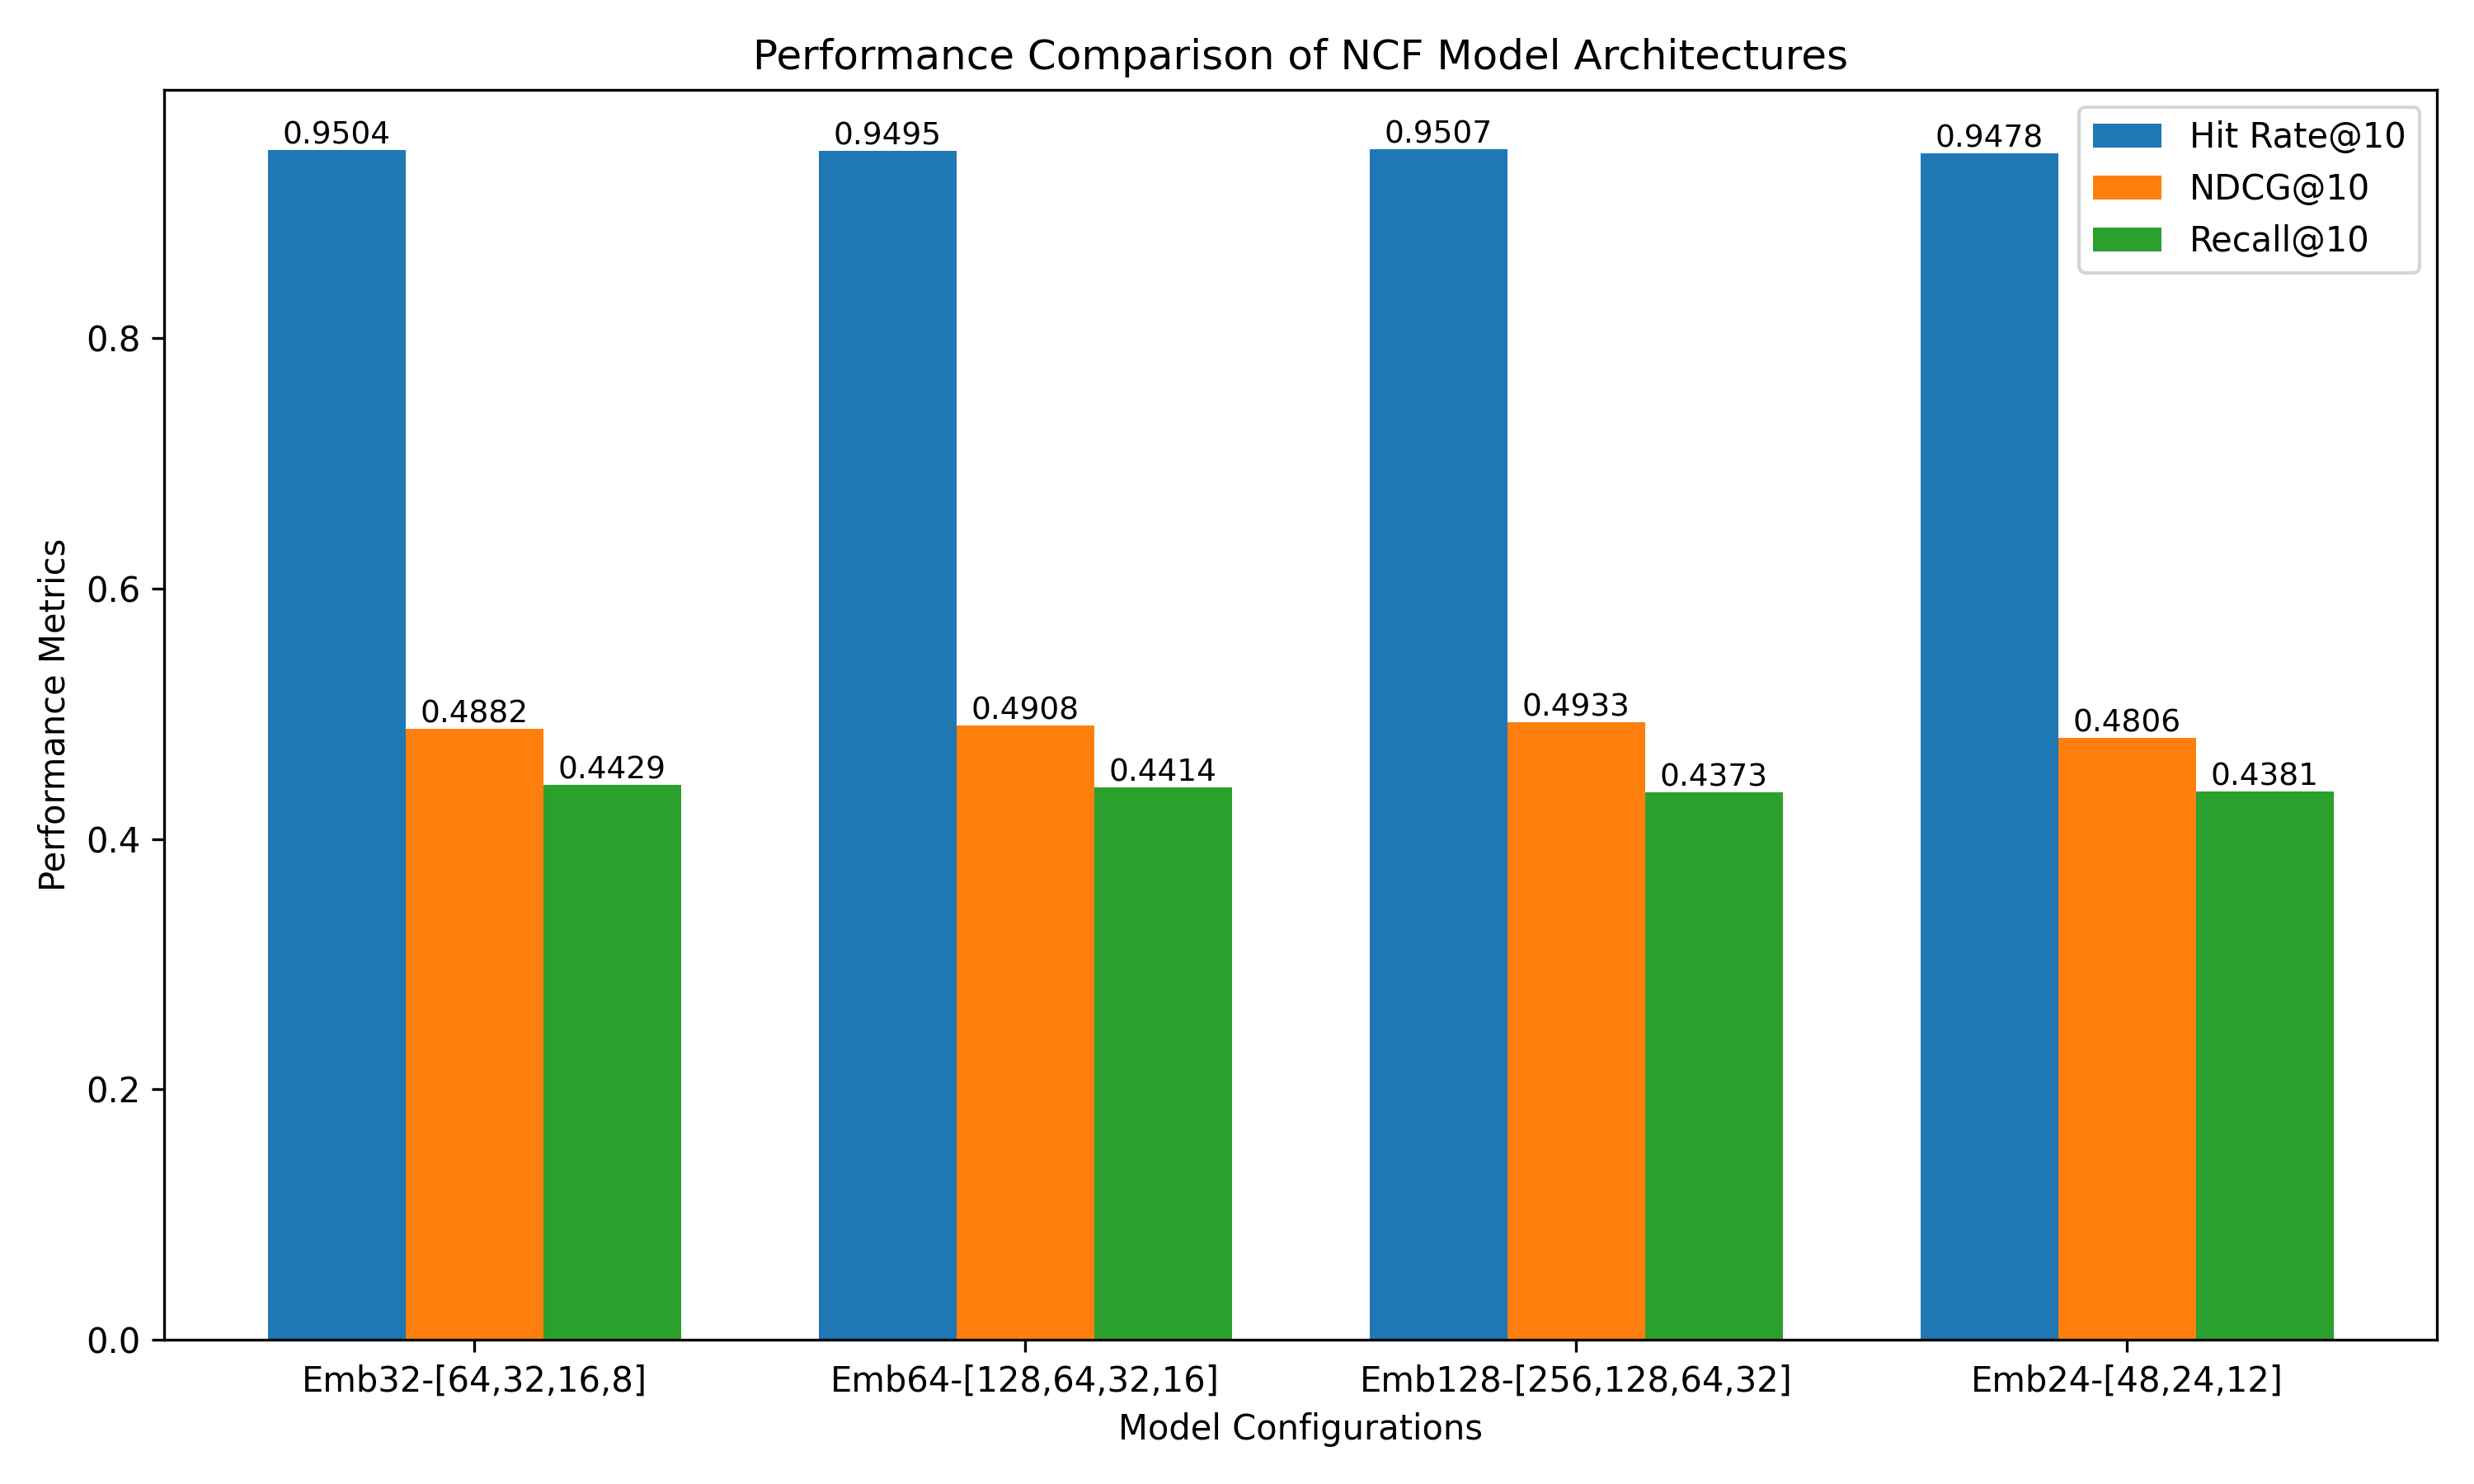
\includegraphics[width=0.5\textwidth]{model_comparison.png}
    \caption{Performance Comparison of NCF Model Architectures Across Embedding Dimensions}
    \label{fig:model_architectures}
\end{figure}

\begin{figure}[h!]
    \centering
    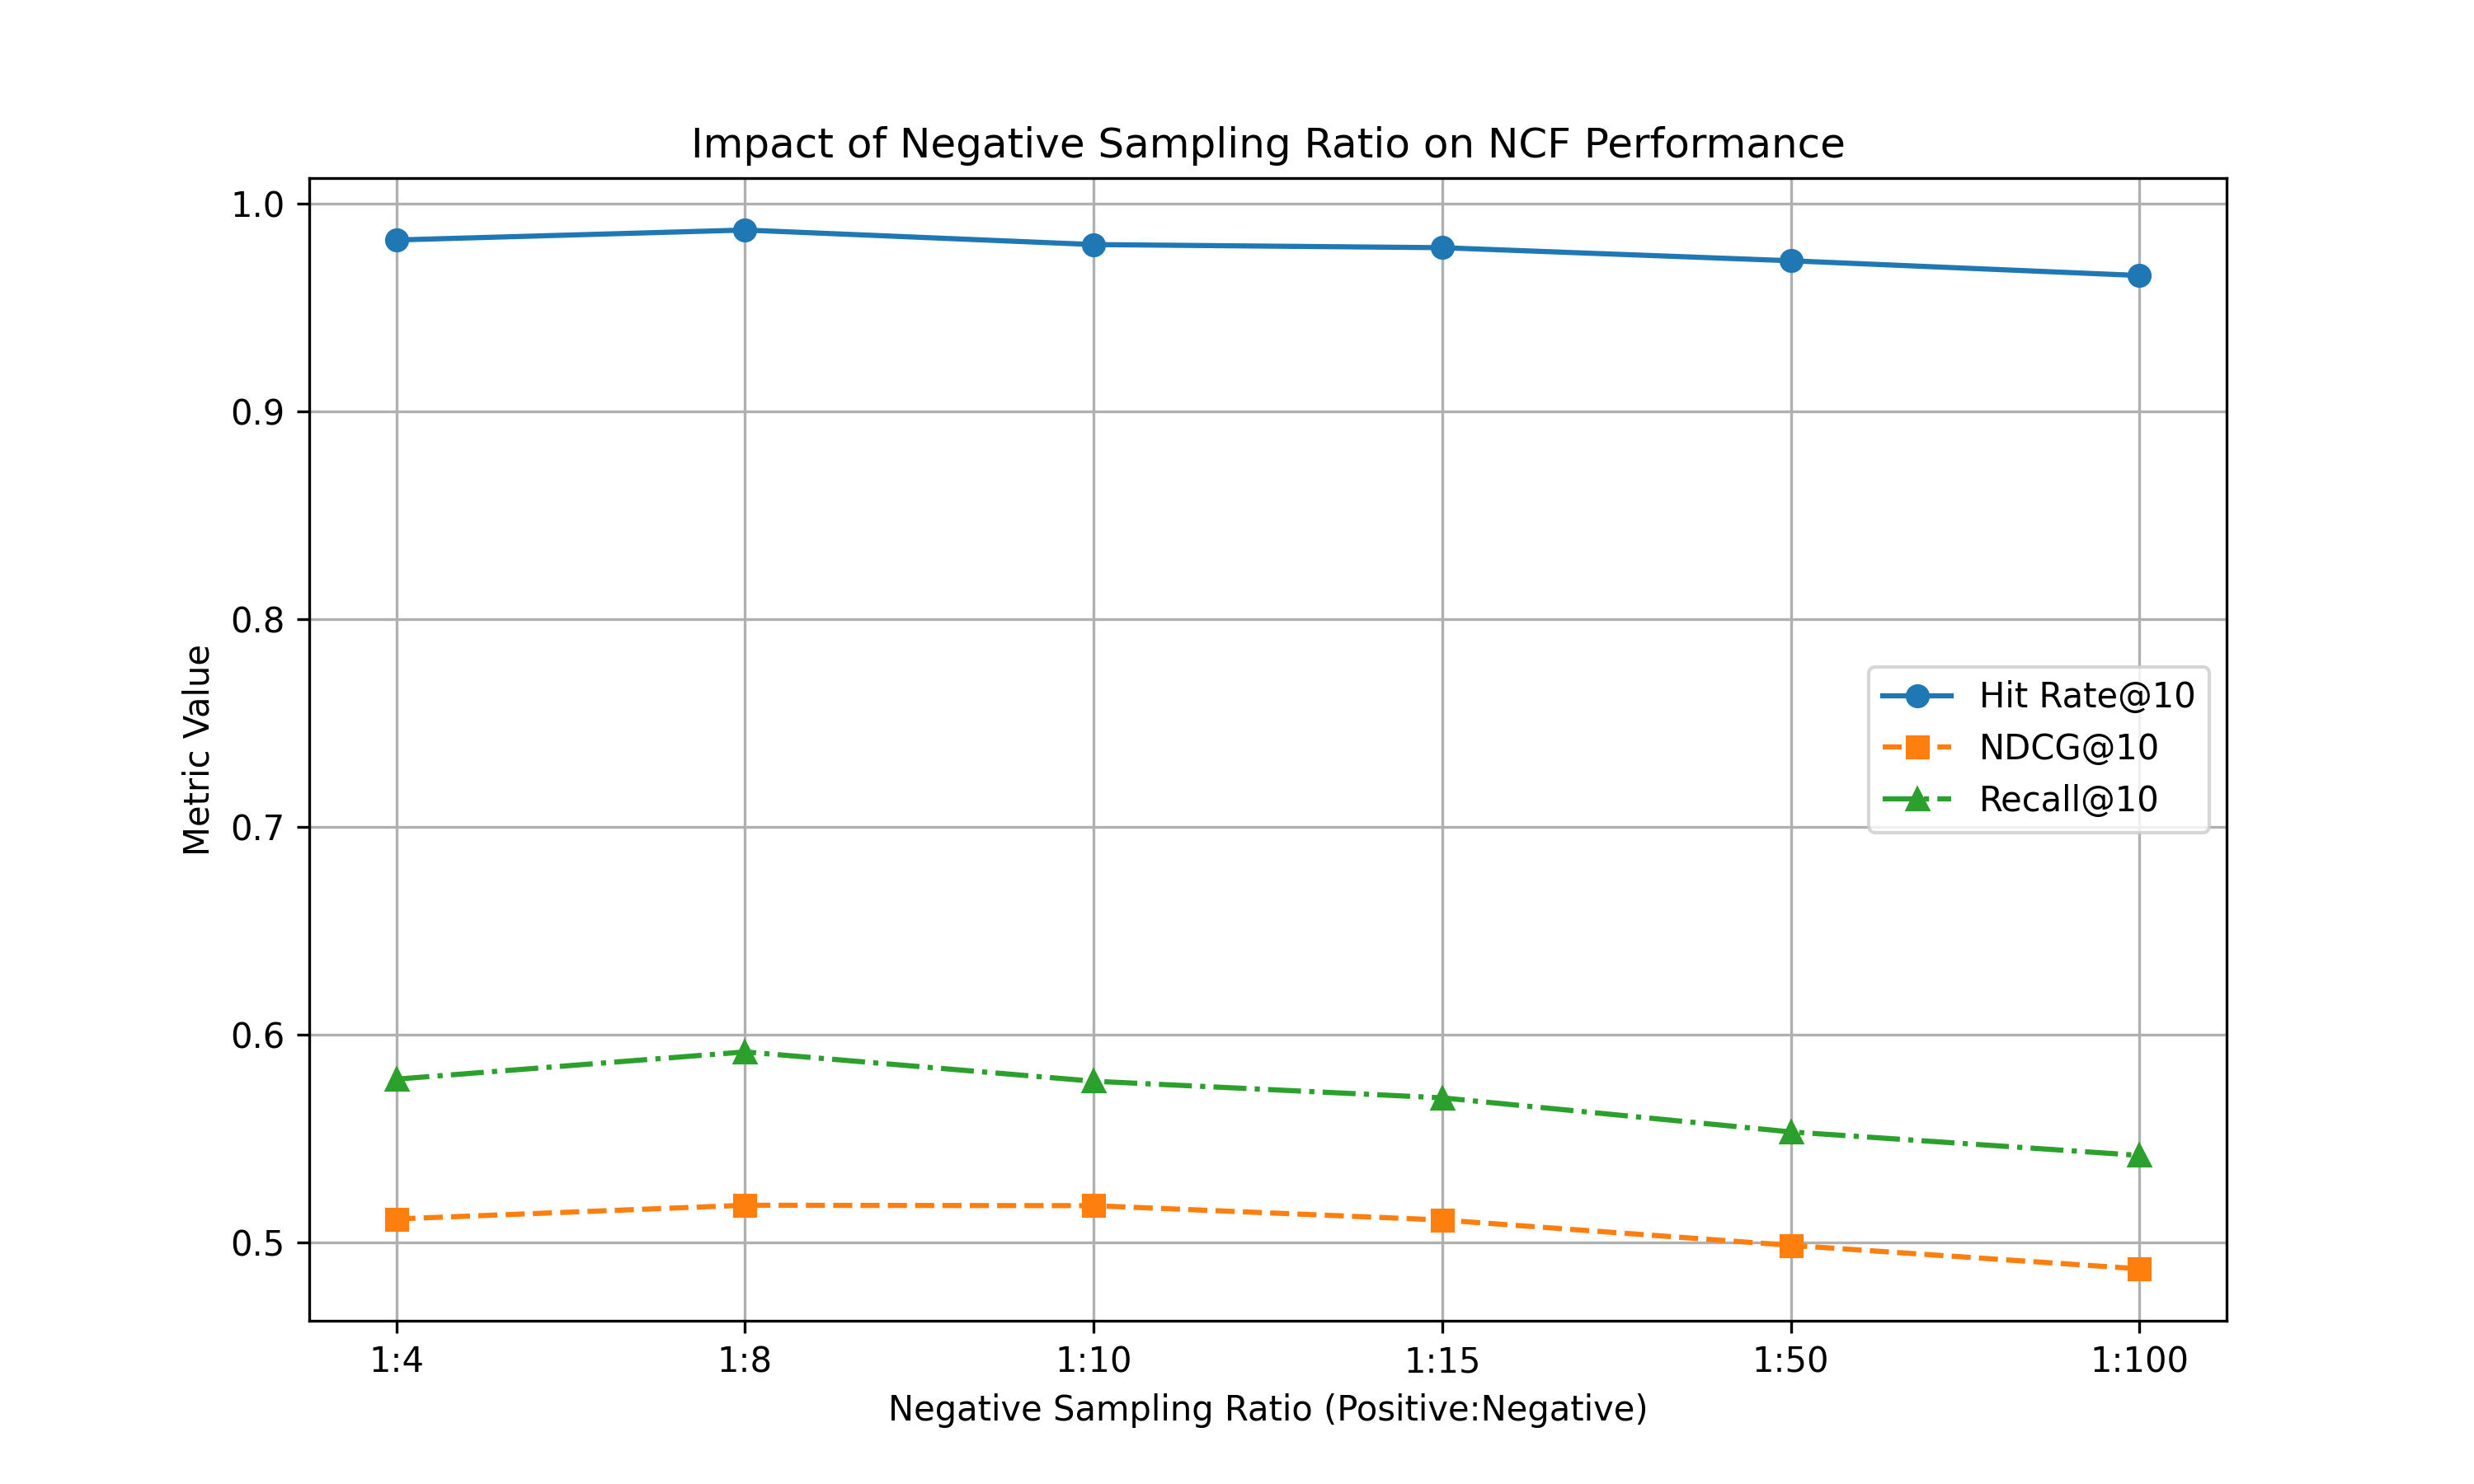
\includegraphics[width=0.5\textwidth]{negative_sampling_ablation.png}
    \caption{Impact of Negative Sampling Ratios on NCF Performance Metrics}
    \label{fig:negative_sampling}
\end{figure}

\end{document}
